\documentclass[11pt]{article}
\usepackage[margin=1in]{geometry}
\usepackage{amsmath,amssymb,amsthm,mathtools,bm}
\usepackage{mathrsfs}
\usepackage{tikz}
\usepackage{pgfplots}
\pgfplotsset{compat=1.18}
\usetikzlibrary{arrows.meta,calc,intersections,decorations.markings}

\title{From Complex Tori to Elliptic Curves via the Weierstrass $\wp$-Function}
\author{}
\date{}

\theoremstyle{definition}
\newtheorem{definition}{Definition}
\newtheorem{exercise}{Exercise}
\theoremstyle{plain}
\newtheorem{theorem}{Theorem}
\newtheorem{proposition}{Proposition}

\newcommand{\C}{\mathbb{C}}
\newcommand{\Z}{\mathbb{Z}}
\newcommand{\CP}{\mathbb{CP}}
\newcommand{\dd}{\,\mathrm{d}}
\newcommand{\wt}{\widetilde}
\newcommand{\wpfn}{\wp}
\newcommand{\disc}{\Delta}

\begin{document}
	\maketitle
	
	\section*{0. Setup}
	Fix a lattice \(\Lambda=\Z\omega_1+\Z\omega_2\subset\C\) with \(\Im(\omega_2/\omega_1)>0\).
	The complex torus is \(X=\C/\Lambda\); write the class of \(z\in\C\) as \([z]\in X\).
	
	\medskip
	\noindent\textbf{Figure 1. Lattice, periods, and a fundamental parallelogram.}
	
	\begin{center}
		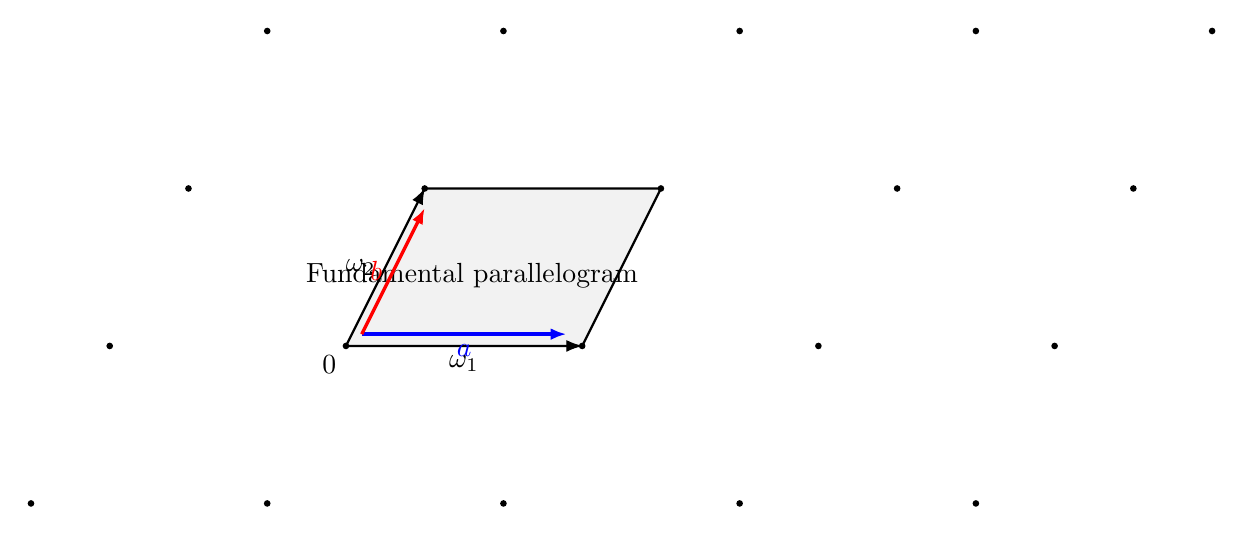
\begin{tikzpicture}[scale=1.0]
			% lattice basis
			\coordinate (O) at (0,0);
			\coordinate (w1) at (3,0);                 % \omega_1
			\coordinate (w2) at (1,2);                 % \omega_2 (tilted)
			% fundamental parallelogram
			\draw[thick,fill=gray!10] (O) -- ($(O)+(w1)$) -- ($(O)+(w1)+(w2)$) -- ($(O)+(w2)$) -- cycle;
			% edges labels
			\draw[-{Latex[length=2mm]}] (O) -- (w1) node[midway,below] {$\omega_1$};
			\draw[-{Latex[length=2mm]}] (O) -- (w2) node[midway,left] {$\omega_2$};
			% lattice points grid
			\foreach \i in {-1,...,3}{
				\foreach \j in {-1,...,2}{
					\fill ($(O)+\i*(w1)+\j*(w2)$) circle (1.2pt);
				}
			}
			% labels
			\node[below left] at (O) {$0$};
			\node at ($(O)+(1.6,0.9)$) {Fundamental parallelogram};
			% cycles a,b
			\draw[very thick,blue,-{Latex[length=2mm]}] (0.2,0.15) -- ++(2.6,0) node[midway,below,blue] {$a$};
			\draw[very thick,red,-{Latex[length=2mm]}] (0.2,0.15) -- ++(0.8,1.6) node[midway,left,red] {$b$};
		\end{tikzpicture}
	\end{center}
	
	\section*{1. Why nonconstant holomorphic functions don't exist on compact Riemann surfaces}
	\begin{proposition}[Maximum principle]
		If \(X\) is compact and \(f:X\to\C\) is holomorphic, then \(f\) is constant.
	\end{proposition}
	\begin{proof}[Sketch]
		On compact \(X\), \(|f|\) attains a maximum. A holomorphic function with an interior maximum is constant. Equivalently, \(\Re f\) and \(\Im f\) are harmonic and attain maxima/minima, hence are constant.
	\end{proof}
	
	\noindent\emph{Moral.} To get nontrivial functions on a compact surface (e.g.\ a torus), we must allow poles: \textbf{meromorphic} functions.
	
	\section*{2. Function fields: the warm-up \(\CP^1\)}
	On \(\CP^1\), the function field is \(\C(x)\): every meromorphic function is a rational expression in a single generator \(x\) (with a pole at \(\infty\)).
	
	\section*{3. The basic elliptic function $\wp$}
	\begin{definition}[Weierstrass \(\wp\)]
		For \(z\in\C\),
		\[
		\wpfn(z)=\frac{1}{z^2}+\sum_{\omega\in\Lambda\setminus\{0\}}\left( \frac{1}{(z-\omega)^2}-\frac{1}{\omega^2}\right).
		\]
	\end{definition}
	\noindent Key properties:
	\begin{itemize}
		\item \textbf{Doubly periodic:} \(\wpfn(z+\omega)=\wpfn(z)\) for all \(\omega\in\Lambda\).
		\item \textbf{Parity:} \(\wpfn\) is even, \(\wpfn'\) is odd.
		\item \textbf{Poles:} a double pole at each \(\Lambda\)-point and no other singularities.
		\item Descends to a meromorphic function \(X\to\CP^1\).
	\end{itemize}
	
	\section*{4. Invariants and the cubic relation}
	Define Eisenstein invariants
	\[
	g_2=60\!\!\sum_{\omega\in\Lambda\setminus\{0\}}\!\!\frac{1}{\omega^4},
	\qquad
	g_3=140\!\!\sum_{\omega\in\Lambda\setminus\{0\}}\!\!\frac{1}{\omega^6},
	\]
	and discriminant \(\disc=g_2^3-27g_3^2\neq0\).
	Then
	\[
	\big(\wpfn'(z)\big)^2=4\big(\wpfn(z)\big)^3-g_2\,\wpfn(z)-g_3.
	\]
	Set \(x=\wpfn(z)\), \(y=\wpfn'(z)\); we get the affine cubic
	\[
	y^2=4x^3-g_2x-g_3.
	\]
	
	\section*{5. Function field of the torus}
	\begin{theorem}
		Every meromorphic function on \(X\) is rational in \(\wpfn\) and \(\wpfn'\):
		\[
		\C(X)=\C(\wpfn,\wpfn')\quad\text{with}\quad (\wpfn')^2=4\wpfn^3-g_2\wpfn-g_3.
		\]
	\end{theorem}
	\noindent\emph{Analogy:} \(\CP^1\) needs one generator \(x\); a genus~1 curve needs two generators \(x,y\) with one relation \(y^2=4x^3-g_2x-g_3\).
	
	\section*{6. Embedding \(X\) as a projective cubic (elliptic curve)}
	Define
	\[
	\Phi:X\longrightarrow \mathbb P^2,\qquad [z]\longmapsto [x:y:1]=[\wpfn(z):\wpfn'(z):1].
	\]
	Its image is the smooth cubic
	\[
	E:\quad y^2 z=4x^3-g_2 x z^2-g_3 z^3\subset\mathbb P^2,
	\]
	and \(\Phi\) extends over the poles so that \([0:1:0]\) is the point at infinity. The group law on \(E\) (via chord-and-tangent) matches addition on \(X\) modulo~\(\Lambda\).
	
	\medskip
	\noindent\textbf{Figure 2.} A sample nonsingular cubic \(y^2=4x^3-g_2x-g_3\) with \(g_2=4\), \(g_3=0\) (so \(\disc=64>0\)).
	\begin{center}
		\begin{tikzpicture}
			\begin{axis}[
				axis lines=middle,
				xlabel={$x$}, ylabel={$y$},
				xmin=-1.5, xmax=1.5, ymin=-3, ymax=3,
				ticks=none, width=9cm, height=6cm,
				]
				% upper branch: y = +sqrt(4x^3 - 4x)
				\addplot[smooth, domain=-1.2:-0.001, samples=300]
				{sqrt( max(0, 4*x^3 - 4*x) )};
				\addplot[smooth, domain=0.001:1.2, samples=300]
				{sqrt( max(0, 4*x^3 - 4*x) )};
				% lower branch: y = -sqrt(...)
				\addplot[smooth, domain=-1.2:-0.001, samples=300]
				{-sqrt( max(0, 4*x^3 - 4*x) )};
				\addplot[smooth, domain=0.001:1.2, samples=300]
				{-sqrt( max(0, 4*x^3 - 4*x) )};
			\end{axis}
		\end{tikzpicture}
	\end{center}
	
	\section*{7. Periods, winding, and motivation}
	Let \(\omega=dz\) on \(\C\). Periods over a fundamental parallelogram’s boundary generate \(\Lambda\):
	\[
	\int_a \omega=\omega_1,\qquad \int_b \omega=\omega_2.
	\]
	The logarithmic \emph{winding form} \(\frac{dz}{z}\) on \(\C^\times\) satisfies
	\(
	\frac{1}{2\pi i}\int_\gamma \frac{dz}{z}\in\Z
	\)
	for loops \(\gamma\), recording winding number. On the torus, taking suitable derivatives of the (doubly periodic) Green/Zeta potentials leads naturally to \(\wpfn\) with minimal pole order~2.
	
	\section*{8. Riemann--Roch viewpoint (``why $\wp$ is minimal'')}
	On a genus~1 curve, \(K\sim 0\). For the divisor \(2[0]\),
	\(
	\ell(2[0])=2
	\)
	with basis \(\{1,\wpfn\}\): \(\wpfn\) is the unique (up to affine change) elliptic function with a \emph{double} pole at~0 and no other poles. For \(3[0]\), \(\ell(3[0])=3\) with basis \(\{1,\wpfn,\wpfn'\}\); eliminating gives the cubic relation.
	
	\section*{9. Minimal formula sheet}
	\[
	\wpfn(-z)=\wpfn(z),\quad \wpfn'(z)=-\wpfn'(-z),\qquad
	\wpfn(z+\omega)=\wpfn(z)\ (\omega\in\Lambda),
	\]
	\[
	(\wpfn')^2=4\wpfn^3-g_2\wpfn-g_3,\qquad
	\disc=g_2^3-27g_3^2\neq0,
	\]
	\[
	\C(X)=\C(\wpfn,\wpfn'),\quad
	[z]\longmapsto[\wpfn(z):\wpfn'(z):1]\in E:\ y^2z=4x^3-g_2xz^2-g_3z^3.
	\]
	
	\section*{10. Exercises}
	\begin{exercise}
		Show any elliptic function has as many zeros as poles (with multiplicity) in a fundamental parallelogram.
	\end{exercise}
	\begin{exercise}
		Using the Laurent series of \(\wpfn\) at \(0\), verify it has a double pole with zero residue.
	\end{exercise}
	\begin{exercise}
		Prove that \(\wpfn\) is even and \(\wpfn'\) is odd.
	\end{exercise}
	\begin{exercise}
		Derive the cubic relation by comparing Laurent expansions of \(\wpfn\) and \(\wpfn'\).
	\end{exercise}
	\begin{exercise}
		Check that the point at infinity \([0:1:0]\) is the identity for the group law on \(E\).
	\end{exercise}
	
\end{document}
